\section{Case Study: EMSim}
\label{sec:case_study}
In this section, we demonstrate Parceive by applying it on EMSim, a simulator
for the european soccer championship. EMSim was part of the student assignments
for our Master course on parallel programming. The application simulates every
match of the group and final phase by relying on historical statistics of
matches, teams, and players. The task was to parallelize the sequential
C code, by considering the following steps: (1) the comprehension of EMSim and
its behaviour, (2) the location of hotspots, (3) the identification of
dependencies, and (4) the parallelization of potential code regions with
appropriate libraries. When done, the students were able to upload their source
code on our submission server to check for correctness and speedup. As it
turned out, the biggest challenges were to estimate the load balance and to
identify data dependencies. In the following, we show how Parceive would have
helped the students with both issues.

In listing \ref{listing:playEM}, we present an excerpt of the EMSim code that
contains a major region for parallelism. The shown \texttt{playEM()} function
gets multiple arrays of teams as input, one for each group of the championship.
Herein, the loop in line 7 calls \texttt{playGroup()} for every group, which
plays all group matches between the given teams and returns the first, second,
and third winners. This loop accounts for \textasciitilde60\% of the overall
runtime of an execution. Even though students might spot the loop as a
potential opportunity for parallelism, the crux is to analyze dependencies
between the calls. The first challenge is to understand the pointer arithmetic
in line 10 and 11, which scatter qualified teams to the successor array. The
second challenge is to inspect the (arbitrary deep) call hierarchies for shared
memory accesses.

\begin{lstlisting}[caption=A major region for loop-parallelism in the
EMSim code, label=listing:playEM]
/* play group phase and final phase of an EM */
void playEM(team_t** teams) {
  team_t* successors[NUM_SUCCESSORS] = {0};
  team_t* bestThirds[NUM_GROUPS] = {0};

  // play groups
  for (int g = 0; g < NUM_GROUPS; ++g) {
    playGroup(
      teams + g,
      successors + (g * 2),
      successors + (NUM_SUCCESSORS - (g * 2) - 1),
      bestThirds + g
    );
  }
...
\end{lstlisting}

We applied Parceive on EMSim by tracing the optimized user binaries (gcc
compiler flag \texttt{-og}). Other libraries that are used by EMSim were not
instrumented since we can preclude conflicting accesses with the user
application. The instrumentation framework and the analyses cause an execution
slowdown of factor \textasciitilde 4.4 (20s instead of 4,5s). The produced
trace data has a size of 4.3Mb, where data about memory accesses and function
invocations account for 84\% of the size. After producing the trace database,
we can import it to our visualization and show the resulting views.

The trace view that depicts the EMSim execution is shown on the upper part
of Figure \ref{fig:emsim}. By doing a top-down inspection, it becomes obvious
that \texttt{main()} spends most of the time in the invocation of
\texttt{playEM()}. Within this function call, the execution time is mainly
spent in two loops. The first loop (the one from Listing \ref{listing:playEM})
performs the group phase. The second loop plays the final rounds, starting from
the round of 16 to the final match. 

\todo{put the main purposes for the trace view to the specific place}
\iffalse
When focusing on parallelism, the users can gain two major insights by looking
at the trace view. One insight is the identification of hotspots to tell which
regions of the user application are worth parallelizing them. After some
parallel regions have been chosen, the other insight is to estimate the
resulting load balance.
\fi

Recall the two main purposes of the trace view, identifying hotspots
and estimating load balance. In the case of EMSim, the view indicates the
invocations of \texttt{playGroup()} and \texttt{playFinalRound} as significant
hotspots. Without considering dependencies, a naive strategy could invoke the
single calls by individual threads. Besides limited scalability (there are only
6 calls of \texttt{playGroup()}), this solution results in a non-optimal load
balance since the calls vary in their execution time. But the trace view
exposes another opportunity for parallelism. Both the group matches and the
final matches lead to distinct calls of \texttt{playMatchGeneral()}. Hence,
a second strategy is to use a master-worker pattern for scheduling these calls
tron a thread-pool. The next step for the user is to validate the found
parallelization strategies.

The CCT view supports users with the validation of prospective system
redesigns. We present the resulting view for EMSim in Figure \ref{fig:emsim}.
Notice that only relevant call nodes for the investigated parallelization
strategies are shown by spotting them on the trace view. Beginning with the
first strategy, we are interested in possible data dependencies between the
invocations of \texttt{playGroup()} and \texttt{playFinalMatch()},
respectively. The corresponding analysis (\textit{show deep dependencies})
queries shared accesses among full call hierarchies. It turns out that each
invocation of \texttt{playGroup()} accesses the global variable
\texttt{groupGoals} and each of invocation of \texttt{playFinalMatch()}
accesses the stack variables \texttt{goals1} and \texttt{goals2}.
Furthermore, the cct view enables to localize these memory accesses such that
the dependencies can be investigated and synchronized.

Even though the data dependencies for the first parallelization strategy can
be easily avoided, we focus on the other strategy that put the calls to
\texttt{playMatchGeneral()} in distinct tasks. The respective CCT view is shown
in Figure \ref{fig:emsim}. Performing the same dependency analysis as
before returns no shared memory accesses between the calls. Hence, the user
gained the necessary information to parallelize EMSim by integrating the
master-worker pattern. A student solution achieved a speedup of 6.5 on our
8-core system. Considering the sequential pre- and post-processing regions,
and the control dependent matches of the final phase (e.g., the semi-final has 
to be played before the final), this speedup confirms Amdahl's law. This result
concludes that our views are very helpful to parallelize user applications.

\begin{figure*}[ht!]
	\begin{center}
		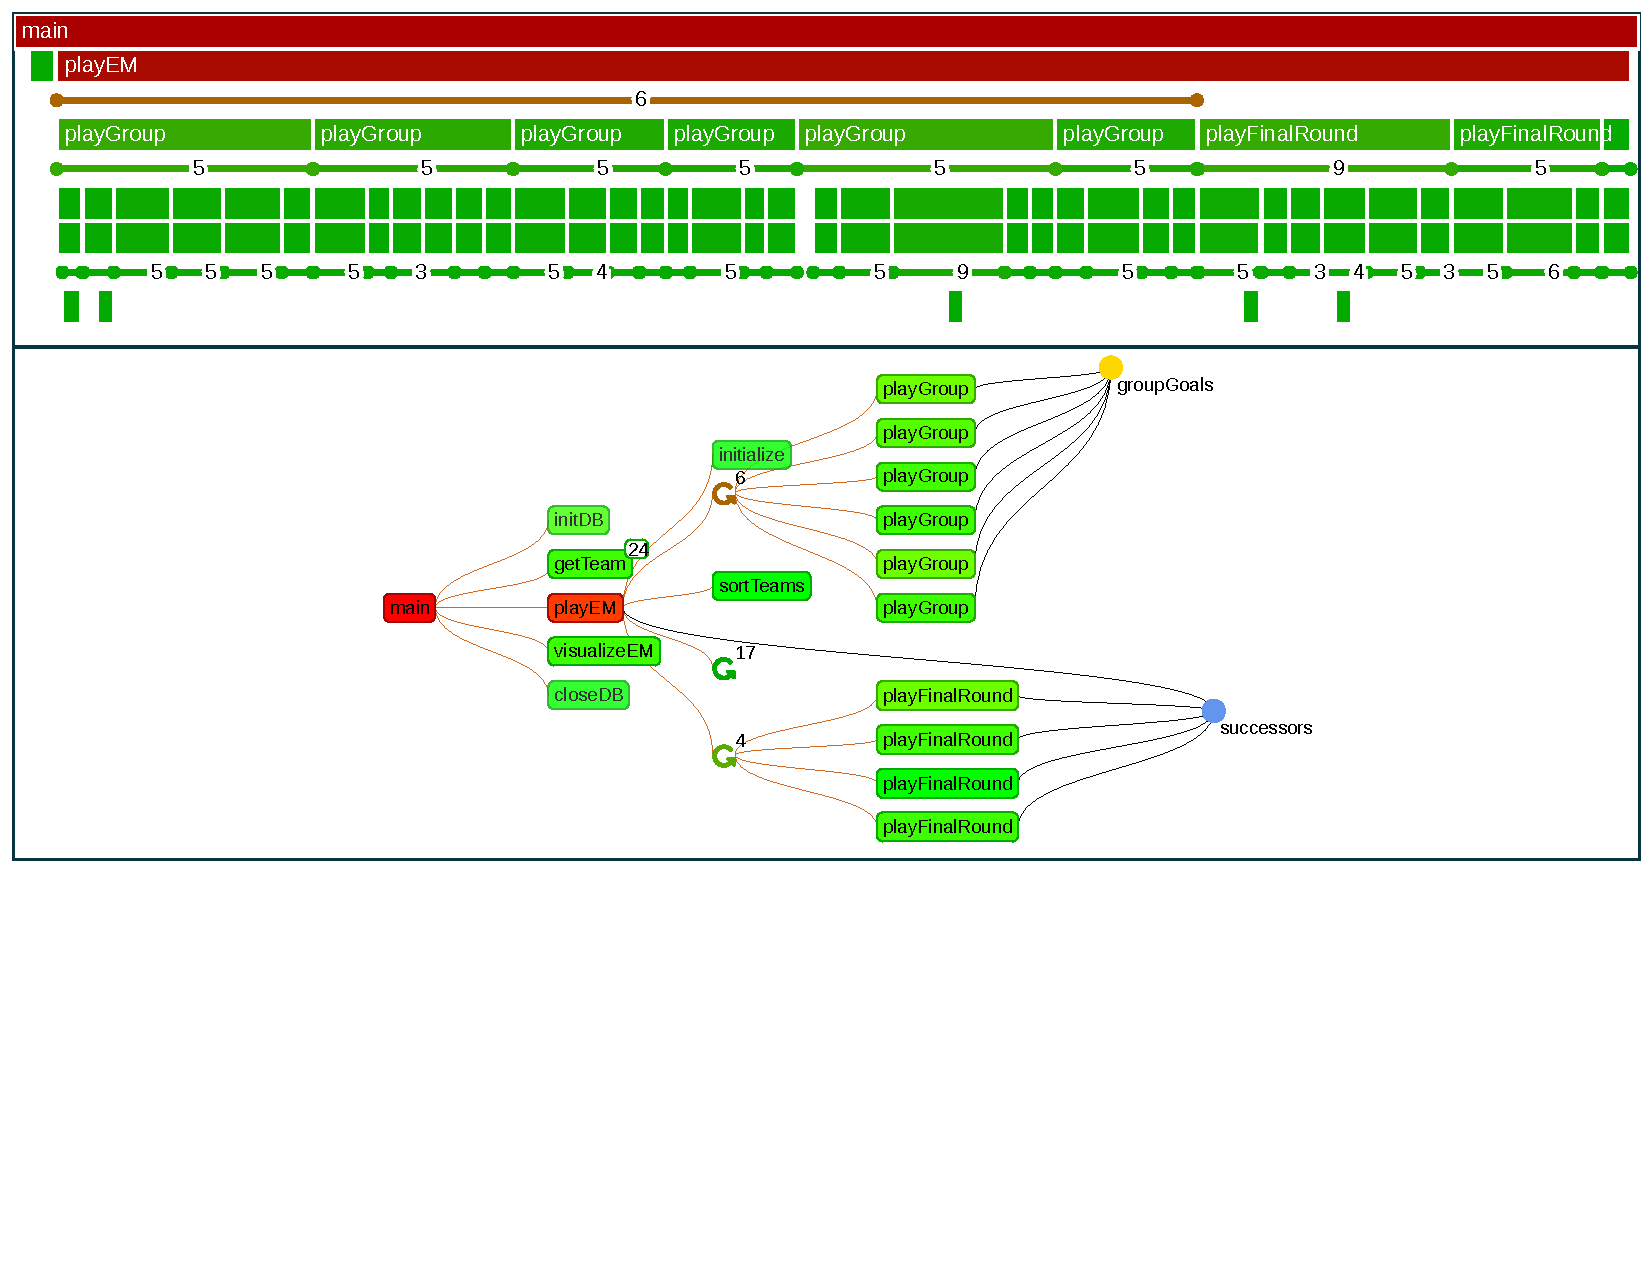
\includegraphics[clip, trim=0cm 7.0cm 0cm 0cm,
width=\linewidth]{img/emsim_overview.pdf}
		\caption{Components of Parceive}
		\label{fig:emsim}
	\end{center}
\end{figure*}
